\documentclass{aastex63}
\usepackage[utf8]{inputenc}
\usepackage{natbib}
\usepackage{listings}
\usepackage{xspace}
\usepackage{paralist}

% for notes support
% \usepackage{geometry}
% \geometry{right=1.5in}

\newcommand{\package}[1]{\texttt{#1}\xspace}
\newcommand{\code}[1]{\texttt{#1}\xspace}
\newcommand{\github}{\package{GitHub}}
\newcommand{\git}{\code{git}}
\newcommand{\python}{\package{Python}}

\newcommand{\sunpyproj}{SunPy project\xspace}
\newcommand{\sunpypkg}{\package{sunpy}}
\newcommand{\sunpycode}[1]{\code{#1}}

\newcommand{\astropy}{Astropy\xspace}
\newcommand{\astropypkg}{\package{astropy}}

\newcommand{\numpy}{NumPy\xspace}
\newcommand{\scipy}{SciPy\xspace}
\newcommand{\matplotlib}{matplotlib\xspace}
\newcommand{\pandas}{pandas\xspace}

\newcommand{\Map}{\sunpycode{Map}}
\newcommand{\Timeseries}{\sunpycode{TimeSeries}}
\newcommand{\Timeseriesmetadata}{\sunpycode{TimeSeriesMetaData}}
\newcommand{\Spectra}{\sunpycode{Spectra}}
\newcommand{\Fido}{\sunpycode{Fido}}
\newcommand{\Lightcurve}{\sunpycode{LightCurve}}
\newcommand{\GenericTimeSeries}{\sunpycode{GenericTimeSeries}}
\newcommand{\GenericMap}{\sunpycode{GenericMap}}

\newcommand{\hpc}{helioprojective Cartesian\xspace}
\newcommand{\hcc}{heliocentric Cartesian\xspace}
\newcommand{\hgs}{heliographic Stonyhurst\xspace}
\newcommand{\hgc}{heliographic Carrington\xspace}
\newcommand{\hpcframe}{\package{HelioprojectiveCartesian}}
\newcommand{\hccframe}{\package{HeliocentricCartesian}}
\newcommand{\hgsframe}{\package{HeliographicStonyhurst}}
\newcommand{\hgcframe}{\package{HeliographicCarrington}}

\shorttitle{SunPy project and v1.0}
\shortauthors{The SunPy Community}

% Words that should not be hyphenated
\hyphenation{NumFOCUS}

% For commenting - can be deleted before submission
%\usepackage[colorinlistoftodos]{todonotes}
%\newcommand{\inlinecomment}[2]{\todo[inline]{#1: #2}\xspace}
%\newcommand{\comment}[2]{\todo{#1: #2}\xspace}

\begin{document}

\title{The \sunpyproj: Open Source Development and Status of the v1.0 Core Package}
\newcommand{\goddard}{NASA Goddard Space Flight Center, Greenbelt, MD 20771, USA}
\newcommand{\catholic}{The Catholic University of America, Washington, DC 20664, USA}
\newcommand{\kharagpur}{Indian Institute of Technology Kharagpur, India}
\newcommand{\Shibpur}{Indian Institute of Engineering Science and Technology Shibpur, India}

\author[0000-0000-0000-0000]{The SunPy Community}
\noaffiliation

% \author[orcid-id]{name}
% \affiliation{}
% below add contributing authors (those folks that have actually worked writing the paper) this list is alphabetical.
% daggers to recognize Stuart, Nabil, Jack, David.
% board members get some symbol next to their names.

\author[0000-0001-9642-6089]{Will T. Barnes}
\affiliation{Lockheed Martin Solar and Astrophysics Laboratory, Palo Alto 94304, CA, USA}
\affiliation{Bay Area Environmental Research Institute, Moffett Field, CA 94952, USA}

\author[0000-0002-5662-9604]{Monica G. Bobra}
\altaffiliation{SunPy Board Member}
\affiliation{W.W. Hansen Experimental Physics Laboratory, Stanford University, Stanford, CA 94305, USA}

\author[0000-0001-6127-795X]{Steven D. Christe}
\altaffiliation{SunPy Board Member}
\affiliation{\goddard}

\author{Nabil Freij}
\altaffiliation{SunPy Deputy Lead Developer}

\author[0000-0002-6835-2390]{Laura A. Hayes}
\affiliation{\goddard}

\author[0000-0002-2019-8881]{Jack Ireland}
\altaffiliation{SunPy Communications Officer, SunPy Board Member}
\affiliation{\goddard}

\author[0000-0003-4217-4642]{Stuart Mumford}
\altaffiliation{SunPy Lead Developer, SunPy Board Member}
\affiliation{SP$^2$RC, School of Mathematics and Statistics, The University of Sheffield, UK}
\affiliation{Aperio Software, Leeds, LS6 3HN, UK}

\author{David Perez-Suarez}
\altaffiliation{SunPy Summer of Code Administrator, SunPy Board Member}
\affiliation{University College London, Gower Street, London, UK}

\author[0000-0001-8661-3825]{Daniel F.\ Ryan}
\affiliation{\goddard}
\affiliation{\catholic}

\author[0000-0001-6874-2594]{Albert Y. Shih}
\affiliation{\goddard}

\collaboration{1000}{(Primary Paper Contributors)}


% Below add contributors to the Sunpy project
% this list is ordered alphabetically
\author[0000-0002-7068-2866]{Prateek Chanda}
\affiliation{\Shibpur}

\author[0000-0002-1361-5712]{Kolja Glogowski}
\affiliation{Kiepenheuer-Institut f\"{u}r Sonnenphysik, Freiburg, Germany}
\affiliation{eScience Department, Computing Center, University of Freiburg, Freiburg, Germany}

\author[0000-0001-8944-4705]{Russell Hewett}
\altaffiliation{SunPy Board Member}
\affiliation{Department of Mathematics, Virginia Tech, Blacksburg, VA 24061-0123}

\author[0000-0003-0787-9559]{V. Keith Hughitt}
\affiliation{Center for Cancer Research, National Cancer Institute, Bethesda, MD 20892-9760, USA}

\author{Andrew Hill}
\affiliation{Oklahoma Baptist University, Shawnee, OK 74804, USA}

\author[0000-0003-3301-1016]{Kaustubh Hiware}
\affiliation{\kharagpur}

\author[0000-0003-0656-2437]{Andrew Inglis}
\affiliation{\goddard}

\author[0000-0001-9874-1429]{Michael S. F. Kirk}
\affiliation{\goddard}
\affiliation{\catholic}

\author{Sudarshan Konge}
\affiliation{Microsoft India Development Center, India}

\author[0000-0002-3783-5509]{James Paul Mason}
\affiliation{\goddard}

\author[0000-0002-4715-1805]{Shane Anthony Maloney}
\affiliation{Astrophysics \&  Space Physics, School of Physics, Trinity College Dublin, Dublin, Ireland}
\affiliation{Astronomy and Astrophysics, Cosmic Physics, Dublin Institute for Advanced Studies, Dublin, Ireland}

% This is not really an affiliation...
\author{Asish Panda}
\affiliation{Google Summer of Code 2014}

\author[0000-0002-1063-9129]{Jongyeob Park}
\affiliation{Space Science Division, Korea Astronomy and Space Science Institute, Daejeon 34055, South Korea}

\author[0000-0003-4747-4329]{Tiago M. D. Pereira}
\affiliation{Institute of Theoretical Astrophysics, University of Oslo, Oslo, Norway}
\affiliation{Rosseland Centre for Solar Physics, University of Oslo, Oslo, Norway}

\author{Kevin Reardon}
\altaffiliation{SunPy Board Member}
\affiliation{National Solar Observatory, Boulder, CO 80303, USA}

\author{Sabrina Savage}
\altaffiliation{SunPy Board Member}
\affiliation{NASA Marshall Space Flight Center, Huntsville, AL 35812, USA}

% may not want to be author, waiting for confirmation
%\author{Kalpesh Krishna}
%\affiliation{University of Massachusetts Amherst}

\author[0000-0002-3713-6337]{Brigitta M.\ Sip\H{o}cz}
\affiliation{DIRAC Institute, Department of Astronomy, University of Washington, Seattle, WA 98195, USA}

\author[0000-0002-1365-1908]{David Stansby}
\affiliation{Department of Physics, Imperial College London, London, SW7 2AZ, UK}

\author{Yash Jain}
\affiliation{\kharagpur}

\author{Garrison Taylor}
\affiliation{Harvard-Smithsonian Center for Astrophysics, Cambridge, MA 02138, USA}

\author{Tannmay Yadav}
\affiliation{\kharagpur}

\author[0000-0003-3552-8799]{Rajul}
\affiliation{\kharagpur}

\collaboration{1000}{(Sunpy Contributors)}

\correspondingauthor{Steven Christe}
\email{steven.christe@nasa.gov}

\begin{abstract}
    The \sunpyproj facilitates and promotes the use and development of several community-led, free, and open source data analysis software packages for solar physics based on the scientific \python environment.
    The project achieves this goal by developing and maintaining the \sunpypkg core package and supporting an ecosystem of affiliated packages.
    The aim of this paper is to describe the first official stable release (v1.0) of the core package as well as the project organization and infrastructure.
    This paper concludes with a discussion of the future of the \sunpyproj.
\end{abstract}

\date{\today}

\section{Introduction}
\label{sec:intro}

Research astrophysicists rely on software to analyze increasingly large and complex data sets.
Scientists that study our nearest star, the Sun, are no different.
Solar physicists rely on remote sensing data from both space- and ground-based instruments to measure the properties of our star and deduce the physical mechanisms at work.
In the past, most solar data analysis was performed using Fortran, a general-purpose, compiled programming language designed for scientific and engineering applications.
Several reasons motivated the solar physics community to transition to the Interactive Data Language (IDL), a commercial and closed-source programming language, in the 1980s.
For one, IDL is an interpreted programming language that enables faster code development compared to Fortran.
Second, IDL includes many libraries that support scientific data visualization and analysis.
Finally, the solar community benefitted from functionality developed by the astronomy community (specifically, the IDL Astronomy User's Library).
Since then, significant functionality was developed by the solar community and freely distributed as the SolarSoftWare library \citep{Freeland:1998we}.

Officially founded in March of 2014, the goal of the \sunpyproj is to provide the core functionality needed for solar data analysis in \python\footnote{\url{https://www.python.org/}}, a high-level interpreted  programming language, and facilitate a new transition to bring significant and new benefits to the solar community.
The \sunpyproj develops and maintains a community-led, free, and open-source\footnote{\url{https://opensource.org/osd}} core \python package (\sunpypkg), supports an ecosystem of affiliated packages (see \autoref{sec:affil_package}) consistent with best practices \citep{Wilson:2014cka}, and engages with the community through mailing lists, chat rooms, tutorials, summer programs, and mentorship.
The \sunpyproj shares these goals with the Astropy Project\footnote{\url{https://www.astropy.org}}, which develops the \astropypkg core package \citep{astropy2018} for the astrophysics community.

The choice of \python was motivated by several different factors.
The scientific \python ecosystem provides a rich and mature ecosystem of packages for performing scientific analysis and computation.
It is supported by foundational packages for manipulating tabular \citep[\pandas,][]{pandas} and multi-dimensional array\citep[\numpy,][]{numpy} data, general purpose scientific computing \citep[\scipy,][]{scipy}, and publication-quality 2D plotting \citep[\matplotlib,][]{matplotlib}\footnote{According to the The 2018 Python Developers Survey \url{https://www.jetbrains.com/research/python-developers-survey-2018/}, data analysis is the primary use for \Python thanks to the broad functionality provided by these foundational packages.}
These core packages form the backbone of hundreds of additional scientific \python packages, such as \astropypkg for functionality and tools specific to astronomy, scikit-learn for machine learning and data mining \citep{pedregosa11}, and Dask for parallel and distributed computing \citep{rocklin15}.
Interoperability between all these packages enables interdisciplinary analysis across traditional fields of study including solar physics, space physics, and astrophysics.

The \python programming language is freely-available, meaning users are not bound by restrictive and costly proprietary licenses.
\python is one of the most widely-used programming languages by professional software developers\footnote{According to the 2019 Stack Overflow developer survey(\url{https://insights.stackoverflow.com/survey/2019}), \python is the fourth most popular language among professional developers.} and is also now used by most universities to teach computer science \citep{guo2014}.
Therefore, early career members of the solar physics community will likely already know how to code in \python.

Finally, an important cultural factor motivated the adoption of \python.
\python and many \python packages are open-source and developed under an OSI-approved open source license.
The \python developer community has embraced an inclusive and open development culture, which means that anyone is welcome to develop functionality to either enhance existing packages such as \sunpypkg or create new ones (see Section \ref{sec:development}).
This means one given person or institution does not control the development of scientific \python software.
Finally, this approach, combined with strict version control, allows scientists to create fully reproducible results.

For all these reasons, the scientific \python ecosystem played a key role in recent major scientific discoveries, such as the first detection of a gravitational wave \citep{ligo_scientific_collaboration_and_virgo_collaboration_observation_2016} and the first image of a black hole \citep{collaboration_first_2019}.
The data and code used to generate these results are openly available, allowing anyone to reproduce these results.
Because the solar community is relatively small\footnote{For reference, out of the $\sim$9,500 members of the American Astronomy Society, approximately 500 are members of the society's Solar Physics Division.} in relation to other scientific communities, it stands to benefit immensely by adopting the \python scientific stack to solve increasingly difficult scientific challenges and produce world-class science.

This paper describes the first stable release (version 1.0) of the (\sunpypkg) core package.
A previous paper describes version 0.5 \citep{Community:2015cy}.
This article is not meant to replace the \sunpypkg documentation but provides an overview of the organization and highlights important functionality.
The full text of the paper, including all of the code to produce the figures, is available in a \github repository\footnote{\url{https://github.com/sunpy/sunpy-1.0-paper}}.

\section{Project Organization and Enhancement Proposals}
\label{sec:proj_org}

The organization of the \sunpyproj is modeled on the structure of a board-only not-for-profit corporate entity.
It consists of an up-to 10 member self-selected board.
An executive director, elected by the board, leads the core development team and the development of the \sunpypkg  package and supports the development of affiliated packages.
As such, the executive director is also referred to as the lead developer.
A deputy lead developer and release manager, as well as other volunteers from the developer community, support the lead developer.
Board members serve two year terms while the lead developer serves one year terms. Both positions have no term limits.

The \sunpyproj is formally defined through SunPy Enhancement Proposals (SEPs), which are modeled after the Python Enhancement Proposal process\footnote{\url{https://www.python.org/dev/peps/}}.
All SEPs are version-controlled, citable, and publicly available\footnote{\url{https://github.com/sunpy/sunpy-SEP}}.
The first SEP \citep[SEP-0001][]{sep-0001} defines the scope of an SEP \citep[similar to][]{ape-0001} while the second \citep[SEP-0002][]{sep-0002} defines the  \sunpyproj organization.

There are generally three types of SEPs:
\begin{itemize}
    \item \textbf{Standard}: Introduces and describes a new feature, or changes to an existing feature to \sunpypkg, and is meant to function as a high-level technical design document.
    \item \textbf{Process}: Describes a new process, or changes to an existing process, in the organization.
    \item \textbf{Informational}: Provides information and does not introduce any new features, changes, or processes.
\end{itemize}

As of the time of writing, there are a total of 9 SEPs which have been approved by the board.
Some notable SEPs have led to the formal adoption of physical units \citep[SEP-0003,][see \autoref{sec:units}]{sep-0003}  and a high precision scientific time format \citep[SEP-0008,][see \autoref{sec:units}]{sep-0008} throughout the code base.
They have also been used to formally define the affiliated package program \citep[SEP-0004,][see \autoref{sec:affil_package}]{sep-0004} and the release schedule and versioning system \citep[SEP-0009,][see \autoref{sec:release}]{sep-0009}.
\section{Support and Sustainability}
\label{sec:support}

To date, the \sunpyproj relies largely on unpaid, volunteer efforts from early career scientists.
The project has not received any significant direct financial support for its work facilitating and promoting open source and open development, including developing the \sunpypkg package itself.
This lack of financial support presents a number of challenges that the \astropy community also faces and have been described in \cite{PriceWhelan:2018ji} and \cite{Muna2016}.

The National Academies of Sciences, Engineering, and Medicine's report on Open Source Software Policy Options for NASA Earth and Space Sciences \citep{NAP2018} outlines several solutions to alleviate these problems -- namely that the NASA Science Mission Directorate provide funding for new and existing open source software projects, promote scientists who spend time developing and improving open source software, and offer prizes for exemplary contributions to the open source software community.
The National Academies of Sciences, Engineering, and Medicine's report on Reproducibility and Replicability in Science \citep{NAP2019} recommends that funding agencies invest in the research and development of open source software that support reproducibility.
The \sunpyproj supports solutions like these for all relevant funding agencies \citep{nas_sunpy_white_paper} and furthermore has the ability to accept financial contributions from institutions or individuals through the NumFOCUS\footnote{\url{https://numfocus.org/}} organization. NumFOCUS is a 501(c)(3) public charity that collects and manages tax-deductible contributions for many open source scientific software packages such as \numpy and \astropy.

The \sunpyproj participates in two summer of code programs, which offer stipends for students to contribute to open source projects.
Since 2013, 16 students have contributed to \sunpypkg and affiliated packages through the Google Summer of Code (GSoC)\footnote{\url{https://summerofcode.withgoogle.com/}} program.
Through a similar program called the ESA Summer of Code in Space\footnote{\url{https://socis.esa.int/}} program, an additional 7 students have contributed since 2011.
Many SunPy community members volunteered to serve as mentors \footnote{\url{https://github.com/sunpy/sunpy/wiki/Wall-of-Fame}}.

\section{Development Model}
\label{sec:development}

To satisfy the mission statement of the Project, the SunPy community adopted an open development model.
This development model is widely used within the scientific Python community.
The \sunpypkg package is hosted on \github and uses \code{git}\footnote{\url{https://git-scm.com/}} as its distributed version control software.
The entire codebase is publicly available and anyone can suggest changes through pull requests.
Since the codebase is licensed under a permissive 2-clause BSD license\footnote{\url{https://opensource.org/licenses/BSD-2-Clause}}, anyone can redistribute, improve, repackage or use it in a closed environment as long as they credit the SunPy developers and redistribute the license.
In order to maintain high quality code, every contribution must satisfy the following requirements:
\begin{enumerate}
    \item Code and documentation must follow widely used style guides (e.g. PEP 8\footnote{\url{https://www.python.org/dev/peps/pep-0008/}}).
    \item All new features must be accompanied with documentation.
    This includes code comments, formal documentation, and gallery examples.
    \item Contributed code must be covered by a test. If the code is not covered by an existing test, a new test or set of tests must be provided.
    \item All code must be within scope. It must be reviewed and accepted by at least two members of the developer community before it is integrated into the codebase\footnote{This requirement is relaxed for bug fixes or small documentation changes.}.
\end{enumerate}
These requirements are imposed on every pull request regardless of contributor.

As of version 1.0, \sunpypkg consists of 48,427 lines of code\footnote{This number includes documentation and comments.
There are 30,906 lines of pure code.} contributed by 123 unique contributors over 11,659 \git commits.
The leftmost panel of \autoref{fig:metafig} shows the steady growth of the code base since 2011 with, on average, approximately 16 lines added per day.
A reduction in the number of lines of code occurred after the release of version 0.9 due to a major clean up effort which led to the deletion of unused code and the removal of support for Python 2.

The middle panel of \autoref{fig:metafig} shows the steady rise in the number of unique contributors with, on average, more than 1 new contributor added each month.
Additionally, the rightmost panel of \autoref{fig:metafig} shows the distribution of total number of commits per contributor as of June 2019.
The distribution is relatively steep with a log-log slope of $-0.34$.
This means that relatively few authors generate the majority of commits.
The top 10 contributors are responsible for close to 80\% of the all commits.

This compares poorly to other projects such as \astropy \citep{astropy2018}.
Unlike \astropy, the \sunpyproj was not formed to bring together and coordinate many existing developers and their \python packages.
The development of the \sunpypkg package began with no prior existing code base by a core group of scientists.
It should be noted that the number of commits is only approximately related to contribution size since a single commit could summarize a substantial increase in functionality or be a simple typographical fix.
Regardless, this distribution suggests that the core developer team has not grown substantially from that original core team.
On the other hand, the total number of unique commits is large which means that there exists a pool of \sunpypkg developers that are willing and have the knowledge to contribute.
Converting these contributors into core developers is crucial to the long-term health of the community.


\begin{figure}
    \center
    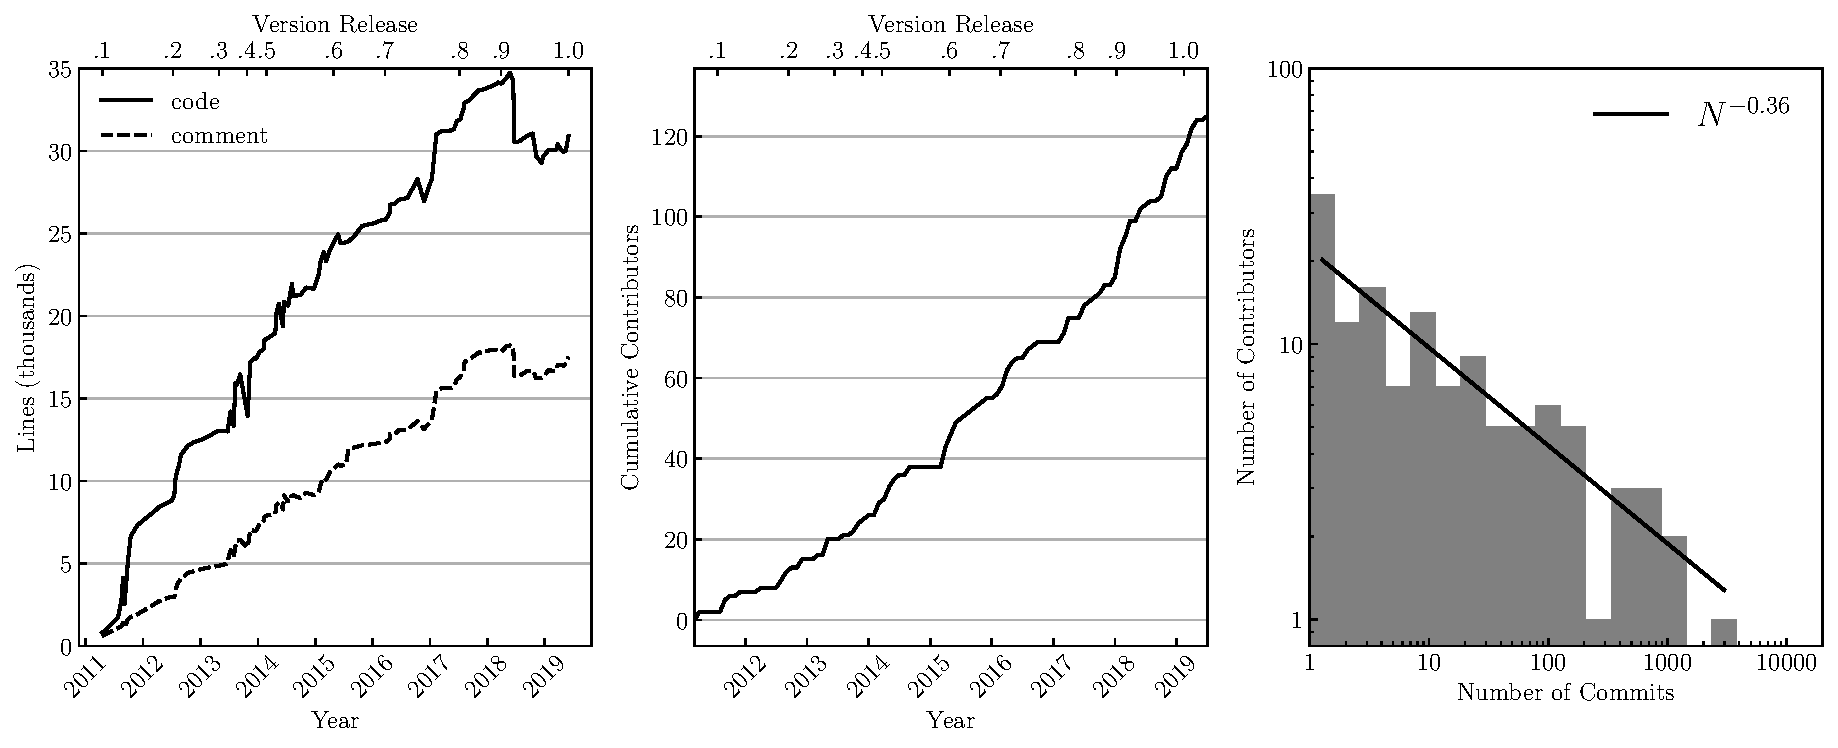
\includegraphics[width = 1.0\textwidth]{figures/dev_meta.pdf}
    \caption{Left panel: A plot of the steady increase in the total number of lines of code (solid line) and documentation line count (dotted line) as a function of time.
	Major releases are indicated.
	A striking reduction in the code base occurred after version 0.9.
	This period saw a major code organization and deletion of obsolete features along with removing support for Python 2.
	Middle panel: The cumulative number of committers (i.e. authors) to \sunpypkg as a function of time shows a steady increase in the number of people involved in the development team.
	Right panel: A plot of the distribution of the number of commits per commiter.
	Though commits is not the best measure this plot does indicates that the majority of commits are undertaken by the least amount of people with an average individual contribution of less than 10 commits.}
\label{fig:metafig}
\end{figure}

\section{The SunPy Core Package}
\label{sec:sunpycore}

The aim of the \sunpypkg package, the core package in SunPy ecosystem, is to provide a set of Python tools for performing common tasks in the analysis of solar data. These include querying and downloading data, loading and visualizing time series and images, and performing coordinate transformations. In the following sections, we describe the primary capabilities of \sunpypkg and highlight several improvements to the package that are included in version 1.0. 

\subsection{Data Search and Retrieval}
\label{sec:fido}

One of the most important tasks that must occur before any analysis can take place is to search for and retrieve data.
A particular science goal may require data from multiple data providers, each of which may have different methods of search and retrieval.
This heterogeneity increases the effort required by scientists to get the data they need.
In order to address this issue, the \package{sunpy.net} subpackage provides interfaces to many commonly used data providers and catalogues in solar physics. 

\subsubsection{The \Fido Interface}
\label{sec:fido}

The most mature and powerful component of \package{sunpy.net} is the \Fido interface for data search and retrieval.
\Fido provides a unified interface that simplifies and homogenizes search and retrieval by allowing data to be queried and downloaded from multiple solar sources simultaneously irrespective of the underlying client.
Currently \Fido supports the Virtual Solar Observatory (VSO), the Joint Science Operations Center (JSOC, see \autoref{sec:drms}) and a number of individual data providers that make their data available via web-accessible resources such as HTTP websites (RHESSI, SDO-EVE, NOAA GOES soft X-ray flux, PROBA2-LYRA and NOAA sunspot number prediction) and FTP servers (NOAA sunspot number, Nobeyama Radioheliograph).

A \Fido search can include multiple instruments, and can query all available data providers with a single query.
Search queries can be made up of many different attributes such as instrument, time range, and wavelength.
The attributes can be joined using Boolean operators to enable complex queries.
The result of a query can be inspected and edited before retrieval.
The result of the \Fido search query is downloaded via asynchronous and parallel download streams.
\Fido also recognizes failed data downloads and allows for re-requesting files which were not retrieved.

\subsubsection{HEK Client}
\label{sec:hek}

In addition to data download, access to event catalogues are also an important aspect of solar physics research.
The primary solar event catalog is the Heliophysics Event Knowledgebase \citep[HEK,][]{hek} which provides a searchable database of manually and automatically detected solar features and events such as sunspots, solar flares, coronal mass ejections, etc. \sunpypkg provides a HEK search client which is highly flexible, allowing multiple event types and their properties to be queried simultaneously.
For example, it is possible to search for SPoCA \citep{2014AA...561A..29V} active regions above a user-specified size within a given time-range.

\subsubsection{Helioviewer Client}
\label{sec:helioviewer}

Finally, \package{sunpy.net} has a Helioviewer\footnote{\url{https://helioviewer.org/}} client which permits the user to query the Helioviewer JPEG2000 image archive, download image data, and easily construct images of solar data from multiple sources available at the Helioviewer archive.
This will eventually be moved out of \sunpypkg to an affiliated package in order to expands the scope of the client.

\subsection{Data Types}
\label{sec:data_types}

The \sunpypkg package provides two core data types that are designed to provide a general, standard, and consistent interface for loading and representing solar data across different instruments and missions.
The two core data types currently provided in \sunpypkg are \Timeseries and \Map, which support 1D temporal data and 2D image data, respectively.
The purpose of these core classes is to standardize data structures regardless of the data source (i.e. observational data from separate instruments).
They maintain a consistent interface for accessing solar data attributes such as the data array itself as well as the metadata and relevant units.
This allows for an easier workflow in the analysis of solar data observations.
These core classes also include functionality for data manipulation and data visualization.
This section provides an overview of the \Timeseries and \Map data types.

\subsubsection{\Timeseries}
\label{sec:timeseries}
Many observations in the field of solar physics consist of time series data.
For example, the X-ray Sensor aboard the Geostationary Operational Environmental Satellite (GOES), which is used as the classification standard for solar flares, continuously measures the disk-integrated X-ray flux as a function of time in two broadband channels.
The \Timeseries class in \sunpypkg aims to accommodate the necessary requirements to represent solar time series data.

\Timeseries allows users to load time series data from a variety of solar instruments and contain the data with appropriate units and time scales (see \autoref{sec:units}).
 A user can create a \Timeseries either from data files stored locally (i.e. observational datasets acquired through \Fido (see \autoref{sec:fido}), or manually from custom time series data.
 The data array as well as the metadata and units data are stored as attributes to the \Timeseries class.

Functionality is also provided for the manipulation of solar time series data.
This includes the ability to add, update, truncate, re-sample and combine data within a \Timeseries or combine multiple \Timeseries together.
\Timeseries also has built-in visualization methods to allow for easy inspection.
An example of a \Timeseries created from GOES X-ray sensor observations during a day for which a solar flare is present is shown in \autoref{fig:timeseries_example}.

\begin{figure}
    \centering
    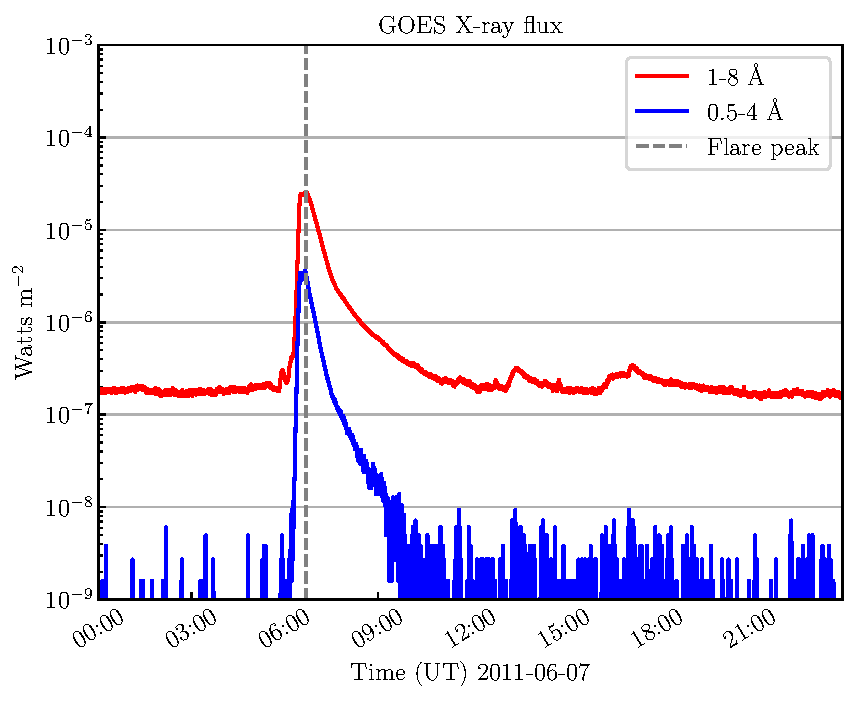
\includegraphics[width=0.55\textwidth]{figures/timeseries_example.pdf}
    \caption{An example of a GOES X-ray Sensor \Timeseries plotted over a 24 hour period. The two colors represent the two broadband channels of GOES 1--8~\AA\ (red) and 0.5--4~\AA\ (blue).  The sharp increase in flux is a solar flare and the grey dashed line denotes the flare peak as found from the Helio Event Knowledgebase (HEK).}
    \label{fig:timeseries_example}
\end{figure}

\Timeseries currently supports the data sources listed in \autoref{tab:instruments} in addition to indices from the National Oceanic and Atmospheric (NOAA) Space Weather Prediction Center (SWPC) that track the solar cycle and its predicted progression. Due to its flexible data structure, it is easy to add additional instruments and data sources to the \Timeseries object.

%%%%%%%%%%%%%%%% TABLE %%%%%%%%%%%%%%%%%%%
\begin{table}
\begin{center}
\begin{tabular}{|p{12cm}|c|c|}
\hline
& \\
\textbf{Supported by \Timeseries}& \textbf{Instrument reference}\\
\hline
\hline
\textit{Geostationary Operational Environmental Satellite (GOES)} X-ray Sensor (XRS) & \citet{garcia94, hanser96} \\
\hline
\textit{Fermi} Gamma-ray Burst Monitor (GBM) &  \citet{meegan2009fermi} \\
\hline
\textit{Nobeyama Radioheliograph (NoRH)} & \citet{nakajima1994nobeyama} \\
\hline
\textit{PRoject for Onboard Autonomy (PROBA2)} Large Yield Radiometer (LYRA) & \citet{dominique2013lyra} \\
\hline
\textit{Solar Dynamics Observatory (SDO)} EUV Variability Experiment (EVE) & \citet{woods2010extreme}  \\
\hline
\textit{Reuven Ramaty High Energy Solar Spectroscopic Imager (RHESSI)} & \citet{lin2003reuven} \\
\hline
 & \\
\textbf{Supported by \Map} & \textbf{Instrument reference} \\
\hline
\hline
\textit{COronal Solar Magnetism Observatory (COSMO)} K-coronagraph (K-Cor) & \citet{dewijn12} \\
\hline
\textit{Hinode} X-Ray Telescope (XRT) & \citet{golub2008x}  \\
\hline
\textit{Interface Region Imaging Spectrograph (IRIS)} Slit Jaw Imager (SJI) & \citet{DePontieu2014}  \\
\hline
\textit{PRoject for Onboard Autonomy (PROBA2)} Sun Watcher using Active Pixel System detector and Image Processing (SWAP) & \citet{seaton2013swap} \\
\hline
\textit{Reuven Ramaty High Energy Solar Spectroscopic Imager (RHESSI)} & \citet{lin2003reuven} \\
\hline
\textit{Solar and Heliospheric Observatory (SOHO)} Extreme ultraviolet Imaging Telescope (EIT) & \citet{delaboudiniere1995eit}\\
\hline
\textit{Solar and Heliospheric Observatory (SOHO)} Large Angle Spectroscopic COronagraph (LASCO) & \citet{brueckner1995large} \\
\hline
\textit{Solar and Heliospheric Observatory (SOHO)} Michelson Doppler Imager (MDI) & \citet{scherrer1995solar}\\
\hline
\textit{Solar Dynamics Observatory (SDO)} Atmospheric Imaging Assembly (AIA) & \citet{lemen2012} \\
\hline
\textit{Solar Dynamics Observatory (SDO)} Helioseismic and Magnetic Imager (HMI) & \citet{schou12}  \\
\hline
\textit{Solar TErrestrial RElations Observatory (STEREO)} Extreme Ultraviolet Imager (EUVI), COronagraph 1 and 2 (COR1/2) for both \textit{STEREO} A and B & \citet{howard2008sun} \\
\hline
\textit{Transition Region and Coronal Explorer (TRACE)}  & \citet{handy99}  \\
\hline
\textit{Yohkoh} Soft X-ray Telescope (SXT) & \citet{tsuneta1991soft}  \\
\hline
\end{tabular}
\end{center}
\caption{The following table outlines the instruments supported by the \Timeseries and \Map objects described in \autoref{sec:data_types}.}
\label{tab:instruments}
\end{table}
%%%%%%%%%%%%%%%% TABLE %%%%%%%%%%%%%%%%%%%

\subsubsection{\Map}
\label{sec:map}
A majority of solar data is in the form images of the Sun.
For example, the Helioseismic and Magnetic Imager (HMI) instrument aboard the Solar Dynamics Observatory (SDO) maps the magnetic field at the solar photosphere across the entire solar disk every 45 seconds with 4k $\times$ 4k pixel resolution.
Image of the Sun are taken in multiple wavelengths from a wide range of both space- and ground- based instruments.
Many high resolution images also require precise coordinate information in order to, for example, compare solar features observed across multiple instruments.

The \Map class in \sunpypkg provides a framework to contain and analyze image data.
A \Map can be created by providing input data files located locally or fetched via the \sunpypkg data search and retrieval interface \Fido (see \autoref{sec:fido}).
The \Map class will automatically detect the instrument of the input data files and parse the metadata to infer the coordinate system from the appropriate FITS keywords \citep{refId0, 2006A&A...449..791T}.
Other source-specific metadata is also used by the \Map class to specify color tables and appropriate image scaling.
It is also possible to create a custom \Map from both a 2D data array and the appropriate metadata, such as coordinate information.

Similar to \Timeseries, the \Map class contains the image data array, coordinate information and relevant metadata as attributes, all of which can be easily accessed by the user.
Visualization methods are also provided to inspect and plot solar image data.
This includes the ability for \Map to plot the image data in a way that represents the world coordinates of the image accurately (see \autoref{sec:coords} for more on solar coordinates).
This allows the user to plot coordinates of interest on a \Map while correctly accounting for the coordinate frame.
Other plotting components in \Map include the ability to mask and clip the image data.

An example of a \Map using data from the Atmospheric Imaging Assembly (AIA) aboard the \textit{Solar Dynamics Observatory (SDO)} is shown in \autoref{fig:map_example}.
The left panel shows the full disk image of the Sun with the relevant image color table and scaling for the observation, and the right panel shows a cropped image in the field of view of the white box in the left panel, highlighting a solar flare.

When analyzing the dynamics of features on the solar disk, it is important to account for variations due to the apparent rotation of the Sun which includes solar differential rotation, a latitudinally-varying rotation rate due to the non-rigidity of the solar interior\citep[see][]{Beck2000}.
The \package{sunpy.physics.differential\_rotation} subpackage provide the ability for a \Map to be transformed to a future time including the effect of solar differential rotation (see \autoref{fig:diff_rot}).

\begin{figure}
    \centering
    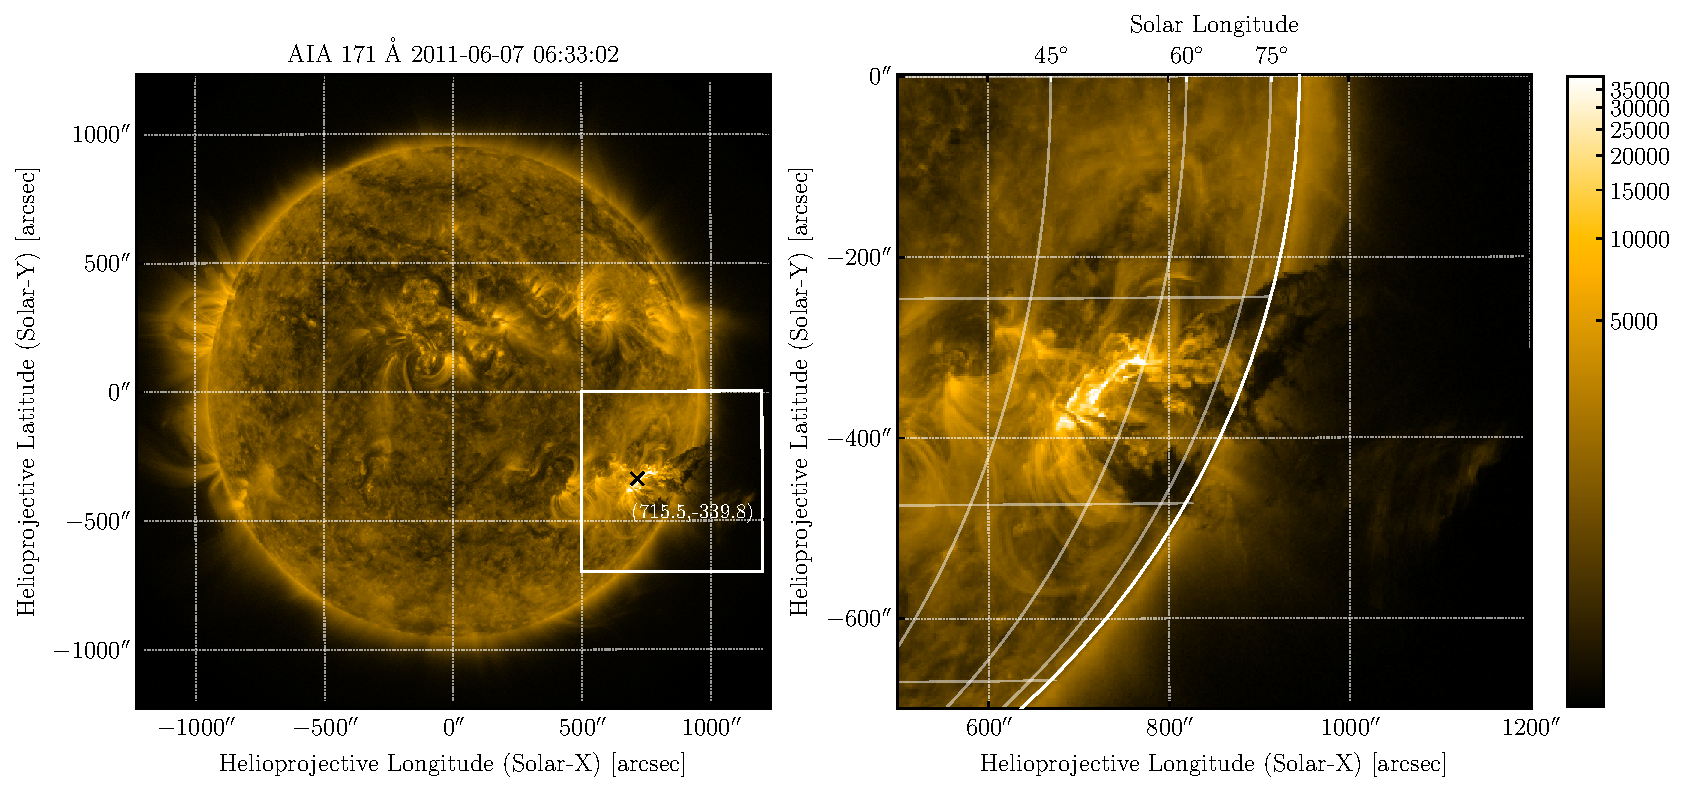
\includegraphics[width=0.97\textwidth]{figures/map_example.pdf}
    \caption{An example of a \sunpypkg \Map plotted from observations of the 171~\AA\ wavelength channel of the Atmospheric Imaging Assembly (AIA) aboard the Solar Dynamics Observatory (SDO).The left hand panel shows a full disk image of the Sun whereas the right hand panel shows a zoom in of the white box in the left hand panel, focusing on the flare that erupted (the same event as the \Timeseries plot in \autoref{fig:timeseries_example}).}
    \label{fig:map_example}
\end{figure}

The \Map class also provides functionality to analyze multiple images, such as overlaying images from different instruments with overlapping fields of view, or to combine multiple images together in a time-ordered sequence.
This includes the ability to co-align images from different instruments or images taken at different times to facilitate multi-instrument studies.


\begin{figure}
    \center
    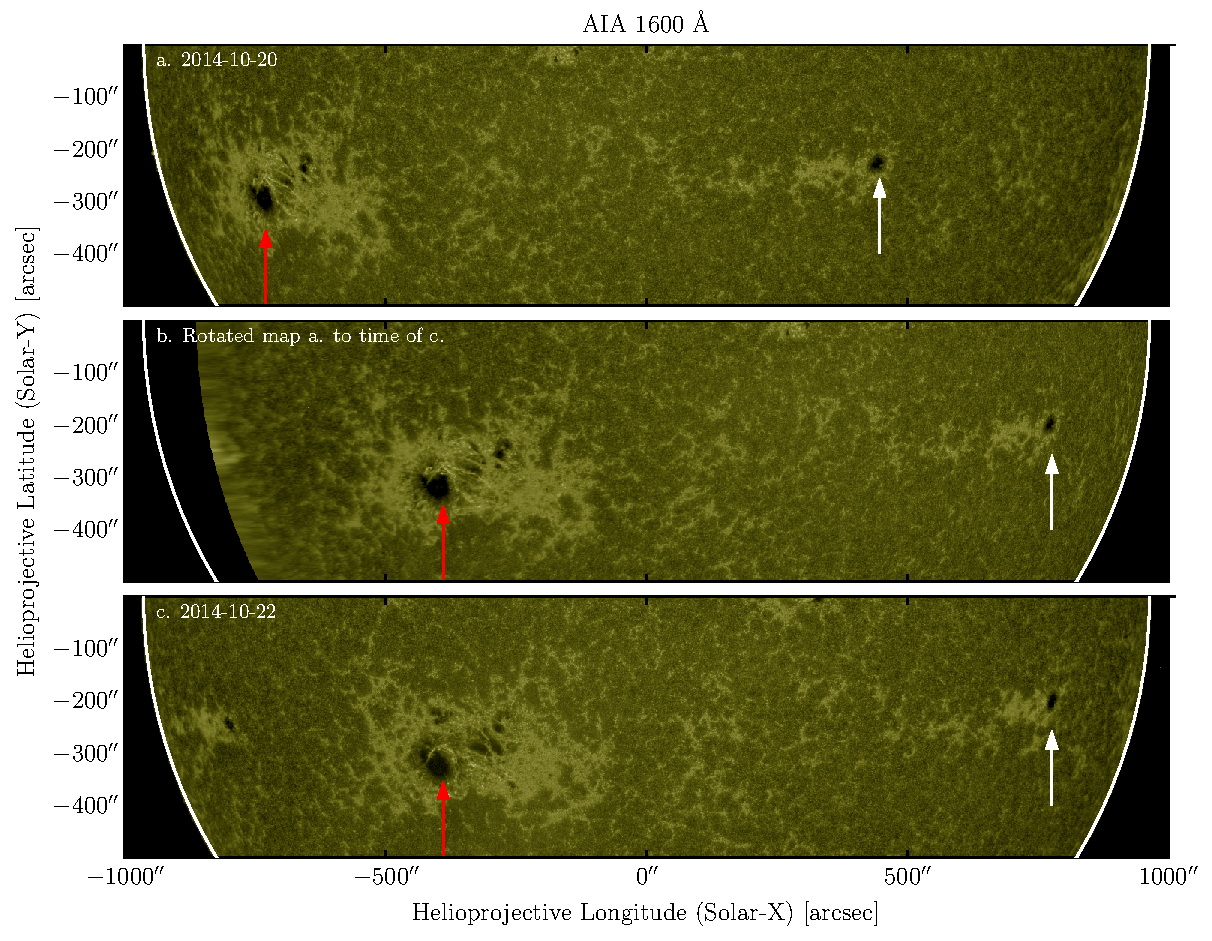
\includegraphics[width = 0.8\textwidth]{figures/fig_diff_rot_1600.pdf}
    \caption{The effects of differential rotation.
    Panels (a) show the Sun as observed by SDO/AIA in 1600~\AA\.
    A large and small sunspot group is highlighted by a red and white arrow respectively.
    Panel (b) shows the predicted image after having been rotated two days into the future.
    Panel (c) shows the actual observation on the day of panel (b) which compares well to the predicted image neglecting the magnetic evolution of the sunspot groups.}
    \label{fig:diff_rot}
\end{figure}

\Map currently supports the data sources listed in \autoref{tab:instruments} as well as the Helioviewer JPEG2000 image files of  each of these data sources. Similar to \Timeseries, \Map is architected to enable new data sources to be added.

\subsection{Solar Coordinates}
\label{sec:coords}

The \package{sunpy.coordinates} subpackage provides support for representing and transforming coordinates used in solar physics.
These coordinates may represent events (e.g., flares), features on or above the Sun (e.g., magnetic loops), or the position of structures traveling throughout the heliosphere (e.g., coronal mass ejections).
The package currently implements many of the most widely used Sun-centered coordinate frames including Helioprojective Cartesian (HPC), Heliographic Carrington (HGC), Heliographic Stonyhurst (HGS),  as well as Heliocentric Aries Ecliptic (HAE), Heliocentric Cartesian (HCC), and Heliocentric Earth Equatorial (HEEQ).
See \citet{2006A&A...449..791T} for more information about each of these coordinate frames.
Additional coordinate frames will be available in future releases.
The functionality provided in this package is built on top of and integrates with the \package{astropy.coordinates} framework \citep[see Section 3.3 of][]{astropy2018}.

An important feature of some of these solar coordinate frames is that they are observer-dependent, meaning that they are not fully defined without also specifying the location of the observer.
The HPC frame, in particular, which is the most widely used coordinate frame for images of the Sun, places the origin of the frame at the observed center of the solar disk.
This means that these observer-dependent frames have axes that change orientation depending on the location of the observer.
The coordinates of the observer are stored in the same object as the other coordinate information.
Since many observations of the Sun take place from or near the Earth, it is frequently an adequate approximation to use the center of the Earth as the observer position.

The observer-independent coordinate frames (HAE, HEEQ, HGC, and HGS) are useful for specifying the locations of features on the Sun or objects (e.g., spacecraft) in interplanetary space.
The commonly-used HGS frame is of particular note because it transforms in a straightforward manner to and from the Heliocentric Celestial Reference System (HCRS).
This reference frame consists of the combination of two rotation angles: the time-independent angle between the Sun's rotation axis and the HCRS celestial pole \citep[see][]{2007CeMDA..98..155S} and the time-dependent angle of the Sun's central meridian (as seen from Earth) relative to the vernal equinox.
The transformation provides the link from the frames defined in \package{sunpy.coordinates} with those defined in \package{astropy.coordinates}, allowing any solar frame to be transformed to and from celestial coordinate frames (see \autoref{fig:transform_graph}).
The functionality provided by the \package{sunpy.coordinates} subpackage has been extensively tested and agrees with published values in the \textit{Astronomical Almanac}.
For example, the apparent right ascension of the Sun agrees to a precision of 0.01 arcsecond.

\begin{figure}
    \centering
    \includegraphics[width=0.75\textwidth]{figures/sunpy_frames.pdf}
    \caption{Diagram of the coordinate frames accessible through \package{sunpy.coordinates}, and how they transform between each other.
    The frames within the blue box are implemented in \package{astropy.coordinates}, but in the shared framework, any frame can be transformed to any other frame in this diagram.}
    \label{fig:transform_graph}
\end{figure}

A few example applications of the \package{sunpy.coordinates} subpackage are shown in \autoref{fig:coordinates_examples}.
The leftmost panel shows magnetic-field-line extrapolations projected onto a SDO AIA 171~\AA{} image of an active region.
The center and rightmost panels of \autoref{fig:coordinates_examples} make use of functions in \package{sunpy.coordinates} to obtain the apparent (light-travel time-corrected) locations of solar-system bodies and overlay them on images of the Sun in solar coordinate frames.

This subpackage also provides the capability to query ephemeris information from a few different sources, including the active ephemeris in \package{astropy.coordinates}, JPL ephemerides, or JPL HORIZONS\footnote{\url{https://ssd.jpl.nasa.gov/?horizons}}.

\begin{figure}
    \gridline{\fig{figures/fig_fieldlines_aia.pdf}{0.3\textwidth}{(a)}
              \fig{figures/fig_venus_transit.pdf}{0.3\textwidth}{(b)}
              \fig{figures/fig_coronagraph_starfield.pdf}{0.3\textwidth}{(c)}
              }
    \caption{Several examples of using the coordinate machinery provided by the \package{sunpy.coordinates} subpackage.
    (a) Magnetic field lines traced from a potential field extrapolation overlaid on an SDO AIA 171~\AA{} observation of an active region from 2019 March 10 00:00:09 UTC.
    The field extrapolation was computed with \package{pfsspy} \citep{david_stansby_2019_3237053}.
    (b) The Venus transit as viewed by SDO AIA in 1600 \AA. The predicted position of Venus is overplotted in the coordinate frame of the AIA image.
    (c) A coronagraph image of the solar corona as observed by STEREO-A COR-2. The predicted positions of stars from the \textit{Gaia} \citep{gaia_collaboration_gaia_2016} Data Release 2 catalog \citep{gaia_collaboration_gaia_2018}, marked by circles, as well as Mars, marked by a box, are overplotted in the coordinate frame of the image.}
    \label{fig:coordinates_examples}
\end{figure}


\subsection{Units and Time Scales}
\label{sec:units}

Solar observations are composed of a physical quantity measured at a specific time.
Specifying physical quantities and time accurately and precisely are therefore fundamental to any solar data analysis task.
In recognition of this, two SEPs have been written to describe the problem, and each mandates a specific solution.

Historically, calculations using physical quantities have been performed in software using raw numbers with no associated units.
At best, the unit information might be provided in a comment or encoded in a variable name.
However, this separation between numbers and units can lead to errors in calculation, which in some cases can have severe consequences\footnote{As an extreme example, the Mars Climate orbiter mission in 1988 failed due to a unit discrepancy \citep{mco_mishap_report}.}.
An effort to minimize the problem of dimensional errors is described in \citet{Damevski2009}, which advocates for the solution to be provided at the software architecture layer.
Following this advice, \sunpypkg utilizes the unit-aware functionality provided by the \package{astropy.units} subpackage throughout the entire code base.
This package provides support for physical quantities through a \code{Quantity} class, which consists of a number and its associated unit(s).
These quantities can be combined in expressions with unit conversions and cancellations automatically taken into account.
Tests have shown that the performance overhead incurred by this functionality is typically minimal.

SEP-0003 \citep{sep-0003} formally mandates that all user-facing functionality provided by \sunpypkg make use of \package{astropy.units}.
All functions and objects must have their input constrained to the appropriate type of unit (e.g. length, mass) and return an error if the input is not correct.
Inputs can then be provided with any appropriate units (e.g. mm, km, inches) and conversions occur automatically without user intervention.
The \package{sunpy.sun.constants} subpackage contains many standard constants relevant to solar physics with additional information such as uncertainty and reference.

Time is another fundamental quantity that must be appropriately specified for scientific uses.
Solar data analysis requires certain functionality to manipulate and represent times and dates.
These requirements include support for leap seconds and the ability to represent, and convert between, specific time scales and formats.
This goes beyond that provided by the standard \python \package{datetime} subpackage.
For this reason, SEP-0008 \citep{sep-0008} was mandated to adopt the use of the \package{astropy.time} subpackage to represent a date or time throughout the \sunpypkg code base.
The \package{astropy.time} subpackage provides the necessary support for non-UTC time scales (such as International Atomic Time (TAI)), and provides functionality for representing common time formats used in solar physics (such as Julian day and Unix time). The \package{astropy.time} object also facilitates custom time formats and scales.
Given that several different time formats and scales are used within solar physics, and in astrophysics alike, it is important to have such a consistent time object with the functionality to convert between different time representations.
This is of particular importance in comparative studies with multi-instrument observations which may use different time measurement systems.
The further advantage of leveraging the functionality of \package{astropy.time} within \sunpypkg is motivated by the support it provides for leap seconds, light travel times, and high precision time representation.
The use of the \package{astropy.time} object also fosters cross-disciplinary studies between solar physics and astrophysics, such as performing detailed timing comparison studies between solar and extra-solar events, and to accurately make use of ephemeris calculations.

\section{Affiliated Packages}
\label{sec:affil_package}

In order to foster collaboration, coordination, and code re-use, the \sunpyproj supports affiliated packages.
These are \python packages that build upon the functionality of the \sunpypkg package and/or provide general functionality useful to solar physics.
Affiliated packages can also be used to develop and mature subpackage functionality outside of the constraints of \sunpypkg for eventual inclusion.
The following requirements must be met by potential affiliated packages:
\begin{itemize}
    \item The package must make use of all appropriate features in \sunpypkg.
    \item Documentation must be provided that explains the function and use of the package, and should be of comparable quality to \sunpypkg documentation.
    \item A test suite must be provided to verify the correct operation of the package.
\end{itemize}
Developers can apply to become an affiliated package to the lead developer with final approval required of the SunPy board.
Packages are re-reviewed on a yearly basis to ensure that they continue to meet the standards.
To enhance discoverability, a list of all affiliated packages is maintained on the SunPy website\footnote{\url{https://sunpy.org/team\#affiliated-packages}} and they are advertised at national and international conferences and workshops.
Finally, the development of these packages is provided informal support by the developer community, and
a package template\footnote{\url{https://github.com/sunpy/package-template}} has been developed that simplifies and standardizes packaging, testing, and documentation.

The following sections provide short descriptions of the existing affiliated packages.

\subsection{drms}
\label{sec:drms}

The \package{drms} package provides functionality to access data hosted by the Joint Science Operations Center (JSOC).
Operated by Stanford, it is the primary data center for SDO/HMI, SDO/AIA, the Solar and Heliospheric Observatory's (SOHO) Michelson Doppler Imager (MDI) instrument, and the NASA Interface Region Imaging Spectrograph (IRIS) Explorer.
This Data Record Management System (DRMS) is based on a PostgreSQL database that contains metadata, as well as pointers to image data, for every image contained in the archive.
The \package{drms} package provides access to query the image metadata in the JSOC DRMS. It can also be used to submit tailored data export requests (e.g. movies and images in various formats) and download data files and is built on the HTTP/JSON interface provided by JSOC.

\subsection{ndcube}
\label{sec:ndcube}

The \package{ndcube} package provides functionality for manipulating N-dimensional coordinate-aware data.
Supports is provided for any combination of axis-types such as images (2 spatial axis), images over time (2 spatial and 1 time axis), spectrograms (wavelength and time), as well as more complex data sets (e.g. slit spectragraphs with wavelength, time, and spatial axes).
The package provides the \sunpycode{NDCube} class, a subclass of \astropy's \sunpycode{NDData} data container that holds together the data array uncertainties, and (potentially) a data mask.
\sunpycode{NDCube} enhances the functionality of \sunpycode{NDData} by adding support for handling world coordinate transformations through the World Coordinate System (WCS) architecture commonly used in solar physics \citep{2002A&A...395.1061G, 2006A&A...449..791T}.
Powerful and intuitive tools are included for slicing datasets with a single command (using either array indices or world coordinates) or slicing all components (including the data array and coordinates simultaneously).
This functionality enables users to manipulate their dataset quickly and accurately, allowing them to more efficiently and reliably achieve their science goals, and is meant to be used as a basis for more advanced and instrument-specific functionality (see \autoref{sec:irispy}).
Support for the generalized WCS module \citep{gwcs2018} is planned for the next major release.

\subsection{radiospectra}
The \package{radiospectra} package supports reading and analyzing dynamic radio spectra, as a function of time, primarily from e-Callisto, the International Network of Solar Radio Spectrometers\footnote{\url{http://www.e-callisto.org}}.
It provides tools for downloading and reading data, handling metadata, homogenizing data, and defining and subtracting background.
This package is planned to undergo major changes with new tools being developed in \code{astropy/specutils}\footnote{\url{https://github.com/astropy/specutils}}.

\subsection{IRISPy}
\label{sec:irispy}

The \package{IRISPy} package provides tools to read, manipulate and visualize data from IRIS, \citep{DePontieu2014}.
IRIS is a NASA Small Explorer mission comprised of two instruments: an imager (SJI) and a rastering slit spectrograph (SG).
\package{IRISPy} is currently limited to reading level 2 data for either of these instruments.
This package provides data classes which hold data from both SJI and SG.
Built on top of the functionality provided by \package{ndcube} (see \autoref{sec:ndcube}). \package{IRISPy} link the main observations, metadata, uncertainties, data unit, mask, and WCS transformations and provides easy slicing of the data in any axis.
Measurement uncertainties accounting for Poisson statistics and readout noise are automatically calculated while a mask is used to ignore bad pixels when performing basic operations (e.g.\ mean, max, and visualizations).

\section{Community}
\label{sec:community}

As discussed in \citet{bangerth2013}, a vital component to the long-term success of a project requires building a healthy community of users, developers, and maintainers.
The \sunpyproj has taken a number of steps to nurture and grow the SunPy community.
We have adopted and enforce a formal code of conduct\footnote{\url{https://docs.sunpy.org/en/stable/code_of_conduct.html}} that strives to foster an open, considerate, and respectful environment for all.
Additionally, we maintain a number of active communication channels including mailing lists, real-time chats based on the open source Matrix protocol\footnote{\url{https://matrix.org}}, and weekly teleconferences.
SunPy community members have also lead tutorials at national and international conferences, participated in summer programs, and provided mentorship to new members of the community.
Developers and contributors are currently provided credit for their work by authorship on papers, posters, and release notes, as well as awards.
For example, in 2018, Vishnunarayan K. I. was presented an award by NumFOCUS for exceptional contributions to the open source scientific software ecosystem by updating \sunpypkg to use \package{astropy.time}.

\subsection{Release Cycle, Versioning, and Long-Term Support}
\label{sec:release}

A formal release schedule for \sunpypkg has been adopted with version 1.0.
The primary goal is to provide clarity for support of releases and to improve predictability of changes to the code base for users of \sunpypkg.
Two releases are planned per year with 6 months between each.
In order to align with the release cycle of \astropypkg, a major dependency for \sunpypkg, the plan is to release each May and November.
The first release of the year will be a Long Term Support (LTS) release, which will be supported for 12 months or until the next LTS release.
The second release will be non-LTS and will be supported for 6 months or until the next release.
The \sunpypkg package will follow an X.Y.z versioning system where the three components have the following meaning:
``X" is the LTS version number (which will be incremented with every LTS);
``Y" is the release counter (which will be 0 for LTS releases and increment for each intermediate non-LTS release);
and ``z" is the bug-fix counter (which will incremented for each bug-fix release).

\section{Infrastructure}
\label{sec:infrastructure}

The \sunpyproj makes use of many tools and web services to develop high-quality code and documentation consistent with best practices.
This section provides an overview of these tools which enable the \sunpyproj to achieve its goals without central institutional oversight.

\subsection{Testing}
\label{sec:continuous-integration}

\sunpypkg's test suite can be broken down into three broad categories: offline, online, and figure tests.
Offline tests are used for checking the majority of the code base.
Online tests specifically test code that makes use of online web services (e.g., VSO, JSOC).
These tests depend on the availability of these online services.
Finally, figure tests are used to ensure that code changes do not unintentionally change plots produced by \sunpypkg.

While the test suite can be run manually, it is important to run the test suite in an automated fashion to maintain the integity of the package and to make it easier for new contributors to understand the impact of their changes.
The \sunpyproj makes extensive use of continuous-integration services, which provide automated testing and code-change inspection.
All proposed code contributions trigger test suites to be run on a number of free services (including
Microsoft's Azure Pipelines\footnote{\url{https://azure.microsoft.com/en-us/services/devops/pipelines/}}, CircleCI\footnote{\url{https://circleci.com}}, and Codecov\footnote{\url{https://codecov.io}}), which integrate into \github.
These services provide the first review of any contribution by running the test suite on each operating system (Windows, Mac, Linux), testing the documentation build, making comparison plots, and providing code-coverage metrics.
Additionally, Travis CI\footnote{\url{https://travis-ci.org}} is used to run the entire test suite on a daily cadence to check for any changes in behavior due to changes in packages that \sunpypkg depends on.

\subsection{Documentation and Gallery}
\label{sec:docs}

The \sunpyproj strives to provide up-to-date, approachable, and high-quality documentation.
All documentation for \sunpypkg, as well as all affiliated packages, uses the \code{Sphinx} documentation build system\footnote{\url{http://www.sphinx-doc.org/en/master/}}.
This system supports using plain text files with a markup language called \code{reStructuredText}.
The build process converts these files, including documentation strings in \python files, into HTML, PDF, or \LaTeX\ documents.
We make use of the \code{sphinx-gallery}\footnote{\url{https://sphinx-gallery.github.io}} extension to build a gallery of analysis examples and the \code{sphinx-automodapi}\footnote{\url{https://sphinx-automapi.readthedocs.io}} extension to generate documentation pages that list all of the available classes, functions, and attributes.
Our online documentation\footnote{\url{http://docs.sunpy.org/en/stable/}} is automatically built and hosted on Read the Docs\footnote{\url{https://readthedocs.org/}} for all releases.

\section{Conclusion}
\label{sec:conclusion}

Development of the \sunpypkg core package has been ongoing for 8 years with the adoption of a formal project structure 5 years ago.
The core package has grown to provide significant and now mature functionality for a growing number of users.
This milestone release of Version 1.0 is in recognition of this achievement, combined with a commitment to stability in future releases.
Significant additional features are currently missing and are either being actively developed or are planned for future development.
These planned udpates include support for generic spectra (one dimensional or multidimensional), multi-dimensional datasets (e.g. slit spectrographs), and a standardized approach to metadata. The roadmap is maintained in a repository\footnote{\url{https://github.com/sunpy/roadmap}} to enable community discussion and suggestions.

The project formalization process, which defined a board structure, has succeeded in providing project stability as well as better recognition in the community.
Through the board, significant decisions were able to be made such as joining NumFOCUS and adopting an official code of conduct\footnote{\url{http://docs.sunpy.org/en/stable/coc.html}}, the purpose of which is to ensure that the SunPy community is positive, inclusive, successful, and growing.

There are a number of obstacles to the continued growth and success of the project. The inability of the project to identify any significant and long-term funding stream has already been discussed in \autoref{sec:support}.
In addition to that challenge, as shown in \autoref{fig:metafig}, the current team of core developers is relatively small, which translates to an unhealthy dependence on key developers.
A significant obstacle to the growth of the core developer team is the difficulty in providing the appropriate tools and guidance to users to convert them into active contributors.
Significant additional skills are required of core developers including knowledge of version control, refactoring code for public use, writing user documentation, and unit testing
These skills are not currently prevalent in the solar community.
The \sunpyproj is considering a number of ways to address this issue, including providing webinars, internship opportunities, and improving online documentation.

The \sunpyproj is now a member of the Python in Heliophysics Community\footnote{\url{heliopython.org}}, whose members contribute to a collection of over fifty \python packages that span every sub-discipline within heliophysics.
\citet{snakes} provides an overview of the current state of \python packages in heliophysics and calls for a common framework to be developed.
The development of \sunpypkg is consistent with the standards established by the community \citep{pyhcStandards} and many members of the \sunpyproj are explicit signatories to these standards.
The goal of this group is to coordinate \python development for heliophysics in order to improve interoperability and efficiency.
In addition, some of the functionality provided by \sunpypkg subpackages may be developed to be generally useful for all of the heliophysics sub-disciplines.

\acknowledgments

We thank the members of the community that have contributed to the \sunpyproj, that have opened issues and provided feedback, and have supported the project in a number of other ways.
Additionally, we thank Brian Dennis, Richard Schwartz, and William Thompson whose comments greatly improved this manuscript.

The following individuals recognize support for their personal contributions.
BMS is supported by the NSF grant AST-1715122 and acknowledges support from the DIRAC Institute in the Department of Astronomy at the University of Washington.
The DIRAC Institute is supported through generous gifts from the Charles and Lisa Simonyi Fund for Arts and Sciences, and the Washington Research Foundation.
DS was supported by STFC studentship ST/N504336/1 and STFC grant ST/N000692/1.

We acknowledge financial contributions from Google as part of the Google Summer of Code program and from the European Space Agency as part of the Summer of Code in Space program.
Additionally, we acknowledge current and future funding from the Solar Physics Division of the American Astronomical Society for SunPy workshops and tutorials at annual meetings.

This work has made use of data from the European Space Agency (ESA) mission \textit{Gaia}\footnote{\url{https://www.cosmos.esa.int/gaia}}, processed by the \textit{Gaia} Data Processing and Analysis Consortium (DPAC)\footnote{\url{https://www.cosmos.esa.int/web/gaia/dpac/consortium}}.
Funding for the DPAC has been provided by national institutions, in particular the institutions participating in the {\it Gaia} Multilateral Agreement.

This research made use of \astropypkg,\footnote{\url{https://www.astropy.org}} a community-developed core Python package for Astronomy \citep{astropy2013, astropy2018}.

\software{
    \astropypkg \citep{astropy_v3.0.5},
    \package{astroquery} \citep{ginsburg_astroquery_2019},
    \package{drms} \citep{Glogowski2019drms},
    \package{GWCS} \citep{gwcs2018},
    \matplotlibpkg \citep{matplotlib_v3.1.0},
    \package{ndcube},
    \numpypkg \citep[v1.14.5][]{numpy},
    \pandaspkg \citep{pandas},
    \package{pfsspy} \citep{david_stansby_2019_3237053},
    \scipypkg \citep{scipy},
    \sunpypkg \citep{sunpy_v1.0.2}
}


\software{Astropy \citep{astropy2018}}

\bibliography{bibliography}

\end{document}
